\section{\ApproachName}
% 我们提出了xxx,通过抽取信息并填充模板的方式来描述节点链接图,它大概分为三个步骤~\REf{}:1. xxx; xxx
We introduce \ApproachName, which describes node-link diagrams by extracting information and filling templates.
\ApproachName~consists of three steps (Figure~\ref{fig:workflow}), which interpret:
\textbf{1) linking conditions} to describe how nodes relationships are constructed by finding, filtering, and sorting conditions;
\textbf{2) visual encodings} by extracting visual mappings among data entities, attributes, visual elements, and visual channels; and
\textbf{3) layout intention} by identifying different kinds of layouts and their affecting factors.

Based on \ApproachName, we implement an interactive interface where creators can input the source code and data to generate node-link diagrams and descriptions.
We augment the generated descriptions by highlight interactions to enhance the comprehensibility.
When audiences hover on different descriptions, relevant parts of the diagram will be highlighted.

\begin{figure}
    \centering
    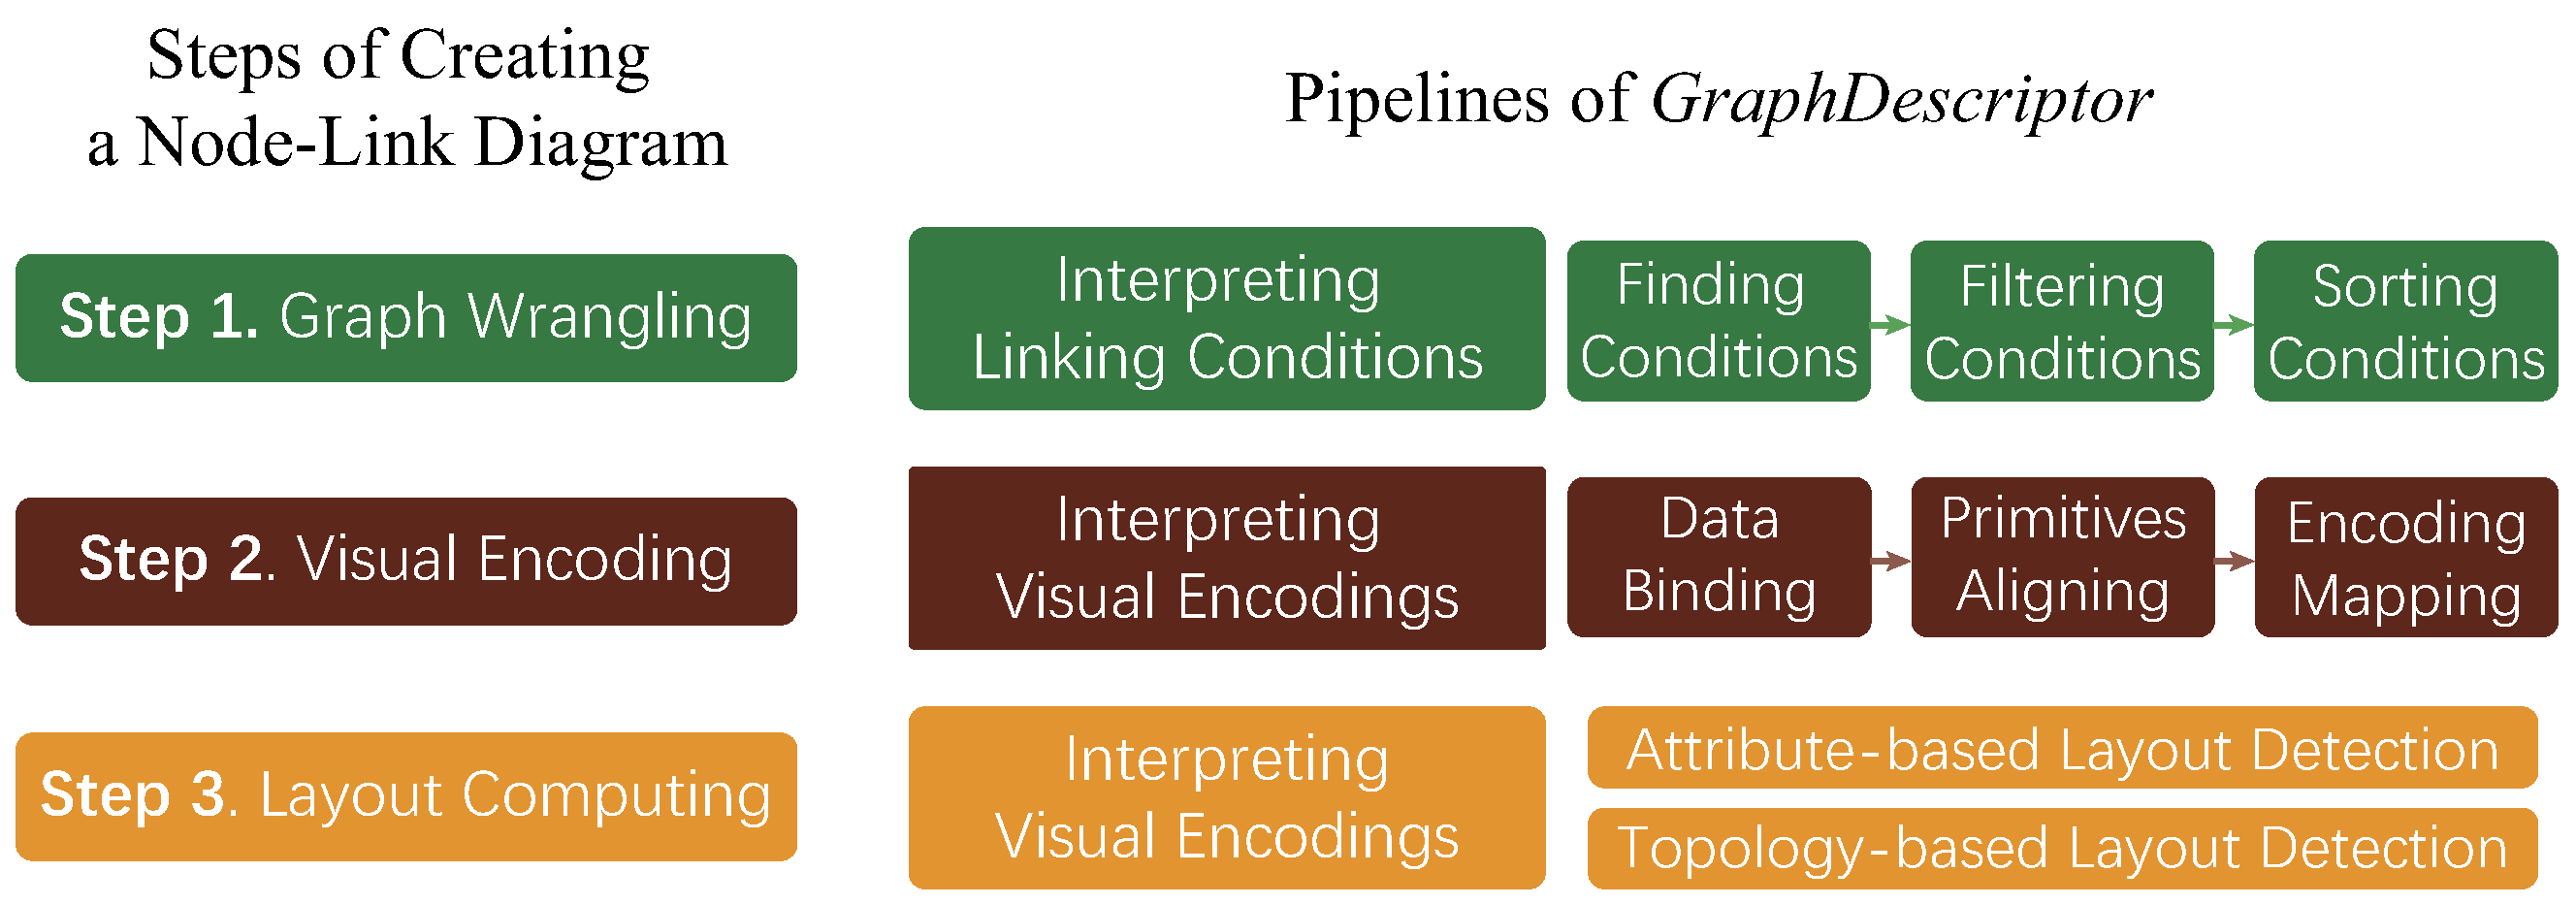
\includegraphics[width=1\columnwidth]{figures/workflow.eps}
    \caption{The pipeline of \textit{\ApproachName} follows the three-step creation process of node-link diagrams to interpret linking conditions, visual encodings, and layout intention.}
    \label{fig:workflow}
\end{figure}


\subsection{Interpreting Linking Conditions}
% 从表格型数据创建图数据时,最重要的就是建立节点之间的关系。
% 观众从节点链接图中所能获知的信息仅仅是某两个节点之间存在联系,但却不了解联系的内在含义。
% 一些论文已经对可能建立链接的情况进行了定义,
Several techniques~\cite{DBLP:journals/ivs/LiuNS14, DBLP:journals/ivs/HeerP14, DBLP:journals/tvcg/SrinivasanPEB18} about graph wrangling identify link construction as the crucial process and propose several linking conditions.
Thus our technique describes linking conditions to interpret the graph wrangling step.
Ploceus~\cite{DBLP:journals/ivs/LiuNS14} and Orion~\cite{DBLP:journals/ivs/HeerP14} infer potential linking conditions by constructing a linking graph and searching valid linking paths. They construct links among multiple data tables by analyzing primary keys and foreign keys.
Graphiti
Graphiti~\cite{DBLP:journals/tvcg/SrinivasanPEB18} identifies potential linking conditions of a homogeneous graph by comparing different attributes.
% 如果多个表合并成一个表,前两者总结的条件可以被Graphiti提出的规则所覆盖
Because multiple tables can be merged into one data table with primary keys and foreign keys, Graphiti can cover the linking conditions by identifying Ploceus and Orion's rules.
Those works infer the potential linking conditions where only a few of links are are constructed. 
% 我们尝试从它们的反方向进行思考,也就是,当我们获取到了所有的链接的时候,推测这些链接是如何被构建的
Whereas, our method runs in the opposite direction where all links have been constructed already.

\textbf{Finding Conditions}. We first construct conditions between all pairs of nodes. Conditions summarized by Graphiti can be organized into four categories:
\begin{compactenum}[\textbf{C1}]
    % 两个节点的某个属性值相同
    \item Values of an attribute of two nodes are the same, e.g., linking two movies published in the same year.
    % 两个节点的某个属性拥有超过一个共同的值
    \item Two nodes have at least one common value of a list attribute, e.g., linking two movies with one or more same actors.
    % 两个节点的某个属性值非常接近
    \item Values of an attribute of the two nodes are significantly close where the significance is defined by the normalized difference.
    \item Values of an attribute of two nodes are in the same bin where the bins are separated by quartiles.
\end{compactenum}

% 为了能够将这些condition填充到文本模板中,我们对condition的输出进行了formalize
We formalize the condition as three aspects to facilitate the comparison, sorting and filtering.
One condition can be defined as:
\begin{equation}
    linking\text{ }condition := ( @type, @attribute, @value )
\end{equation}
Where $@type$ is the condition type, $@attribute$ is the name of the attribute, $@value$ is the value of the attribute.

\textbf{Filtering Conditions}.
We first detect linking conditions held on node pairs without any connections.
These conditions are regarded as false condition because no links are constructed for these nodes and should be filtered out.
We describe our filtering strategy in Algorithm~\ref{alg:conditions}.

\textbf{Sorting Conditions}.
After that, conditions are sorted, so that the highest ranked condition will be regard as the most possible condition.
First, all conditions are sorted by their degrees.
Some conditions are stronger than others.
More stronger conditions are ranked higher than others.
For example, the condition $(@type=C2, @attribute=actors, @value=[Alice, Bob])$ is stronger than $(@type=C2, @attribute=actors, @value=[Alice])$ and $(@type=C2, @attribute=actors, @value=@arbitrary\text{ }value)$, where $(@value=@arbitrary\text{ }value)$ means the condition does not assume the $actors$ attribute should equal to a certain value.
Because the first condition is implied by the latter two conditions,
it is stronger than the others.

We textualize the linking condition of the graph by filling templates. 
Four templates corresponds to four conditions according the $type$:
\begin{compactenum}[\textbf{C}1]
    \item \textit{``Two nodes are connected if the values of the attribute $@attribute$ are the same\$\{ ($@value$)?\}''}.
    \item \textit{``Two nodes are connected if the values of the attribute $@attribute$ have common values\$\{ ($@value$)?\}}''.
    \item \textit{``Two nodes are connected if the values of the attribute $@attribute$ are close (with a difference less than $@value$)''}.
    \item \textit{``Two nodes are connected if the values of the attribute $@attribute$ are within the same \$\{$@value$ ?\}bin''}.
\end{compactenum}
Where \$\{?\} means the included part is optional. 
For example, for Condition \textbf{C2}, two movies are connected because they share same actors Alice and Bob. 
The condition is represented as: $(@type=C2, @attribute=actors, @value=[Alice, Bob])$. 
Its corresponding description is: \textit{``Two nodes are connected if the values of the attribute actors have common values ([Alice, Bob])''}. 
For the condition $(@type=C2, @attribute=actors, @value=@arbitrary\text{ }value)$, contents in the parentheses are omitted.

\begin{algorithm}[!t]
    \renewcommand\arraystretch{1.2}
    \caption{ Filtering Conditions }
    \label{alg:conditions}
    \begin{algorithmic}[1]
        \Require
            $G=(V=\{v_1, v_2, ..., v_n\}, E=\{e_1, e_2, ..., e_n\})$: a graph;
        \Ensure
            $C$: the potential condition set
        \State Init conditions $C=\varnothing$, false conditions $FC=\varnothing$
        \For {each node pair $(v_i, v_j)$}
            \If {$(v_i, v_j)$ is not a link}
                \State $C_{ij} \gets$ all conditions that can link $(v_i, v_j)$
                \State merge $FC$ with $C_{ij}$
            \EndIf
        \EndFor
        \For {each link $e_k=(v_i, v_j)$}
            \State $C_{ij} \gets$ all conditions that can construct link $e_i$
            \For {each condition $c$ in $C_{ij}$}
                \If {$c$ in $FC$}
                    \State remove $c$ from $C_{ij}$
                \EndIf
            \EndFor
            \State merge $C$ with $C_{ij}$
        \EndFor
        \For {each condition $c$ in the condition set $C$}
            \If {the frequency of $c$ is less than $|E|$}
                \State remove $c$ from $C$
            \EndIf
        \EndFor
        \State \Return $C$
    \end{algorithmic}
\end{algorithm}


\subsection{Interpreting Visual Encodings}\label{sec:visualencodings}
\subsubsection{Background}
% 为了在节点链接图中展示节点、链接的属性,常常将这些属性编码为节点/链接的视觉通道。
Creators often encode attributes of nodes and links with visual channels to reveal attribute-based patterns.
For the node-link diagram example in Figure~\ref{fig:VisualEncodings}, a node contains a categorical attribute (\textit{x}) and a numerical list attribute (\textit{y}), we encode the numerical list attribute with two rectangles' height and encode the categorical attribute with two rectangles' fill color and the background rounded rectangle's stroke color.
We denote graphical elements (e.g., \texttt{<circle>}, \texttt{<rect>}, \texttt{<ellipse>}, et cetera) in node-link diagrams as \textit{visual elements} and their style attributes such as \texttt{cx}, \texttt{cy}, \texttt{width}, and \texttt{height} are denoted as \textit{visual channels}.
Nodes and links contained in the underlying graph are denoted as \textit{data entities} and each data entity consists of several \textit{attributes}.

\begin{figure}[ht]
    \centering
    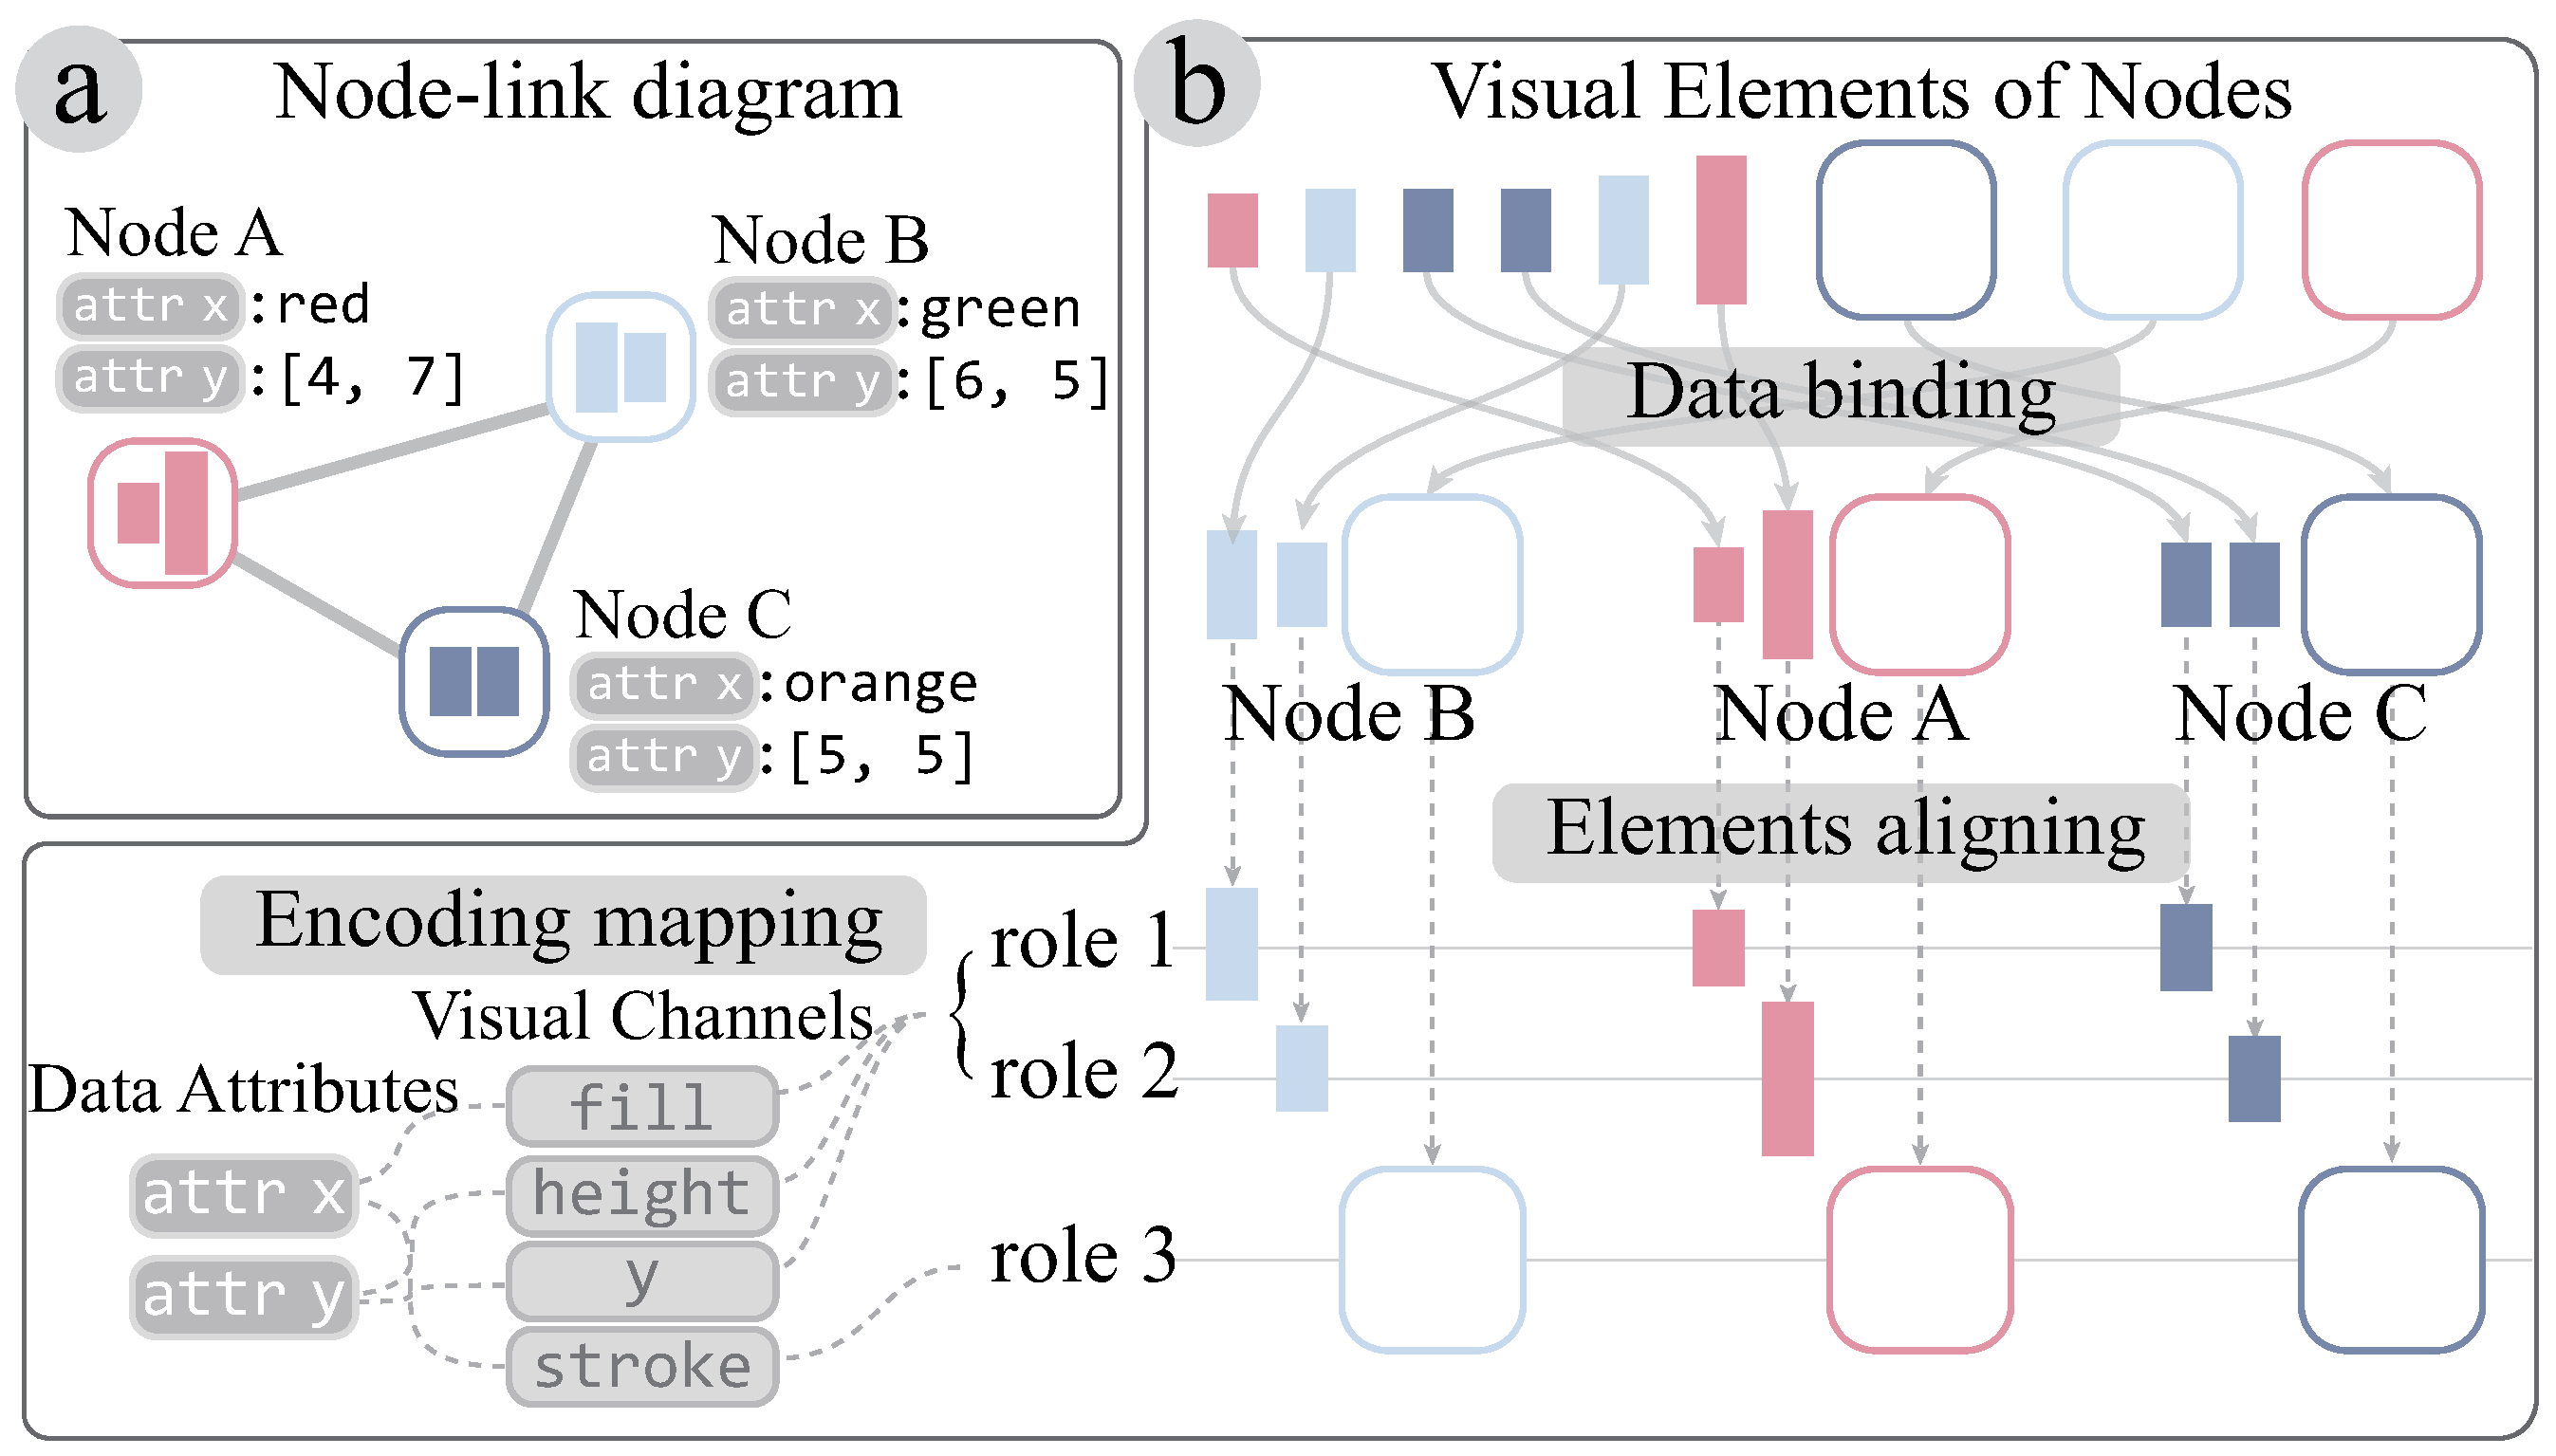
\includegraphics[width=1\columnwidth]{figures/VisualEncodings.eps}
    \caption{An example shows the workflow of our visual encoding extracting technique. A node-link diagram consists of three nodes and three links (upper right corner). Node elements are extracted and the \textbf {data binding} step binds them to different nodes. Then elements with same role across different nodes are aligned into the same role class in the \textbf{elements aligning} step. Mappings among different role calsses, visual channels, and attributes are detected by the \textbf{encoding mapping} step.}
    \label{fig:VisualEncodings}
\end{figure}

% 我们的工作通过分析源代码,从中提取数据实体()是如何被编码为视觉通道的()
We formulate the problem of describing visual encodings in node-link diagrams by three questions:
\begin{compactenum}[\textbf{Q}1]
    \item \textit{What elements does a node/link consists of in the diagram?} For example, in Figure~\ref{fig:VisualEncodings}, a node is composed of three rectangles. \label{qstn:composition}
    
    \item \textit{What attributes do elements and their visual channels encode?} For example, in Figure~\ref{fig:VisualEncodings}, the height of the left rectangle encodes the first item of the attribute $y$. If the shape (\texttt{tagName}) of a element encodes some attribute, we should classify and discuss when elements are encoded into different shapes (e.g., when the node is encoded into a \texttt{<circle>}, the radius encodes its degree, and when the node is encoded into a \texttt{<rect>}, the width and the height encode its degree). \label{qstn:encodings}
    
    \item \textit{Whether there is a certain type of correlation (positive, negative, or categorical) between attributes and visual channels?} e.g., The greater the degree of the node, the greater the radius of the circle.\label{qstn:correlation}
\end{compactenum}
Thus, extracting mappings between entities and elements and correlations between attributes and visual channels are necessary (Figure~\ref{fig:ElementAligning} (a)).


\begin{figure}[ht]
    \centering
    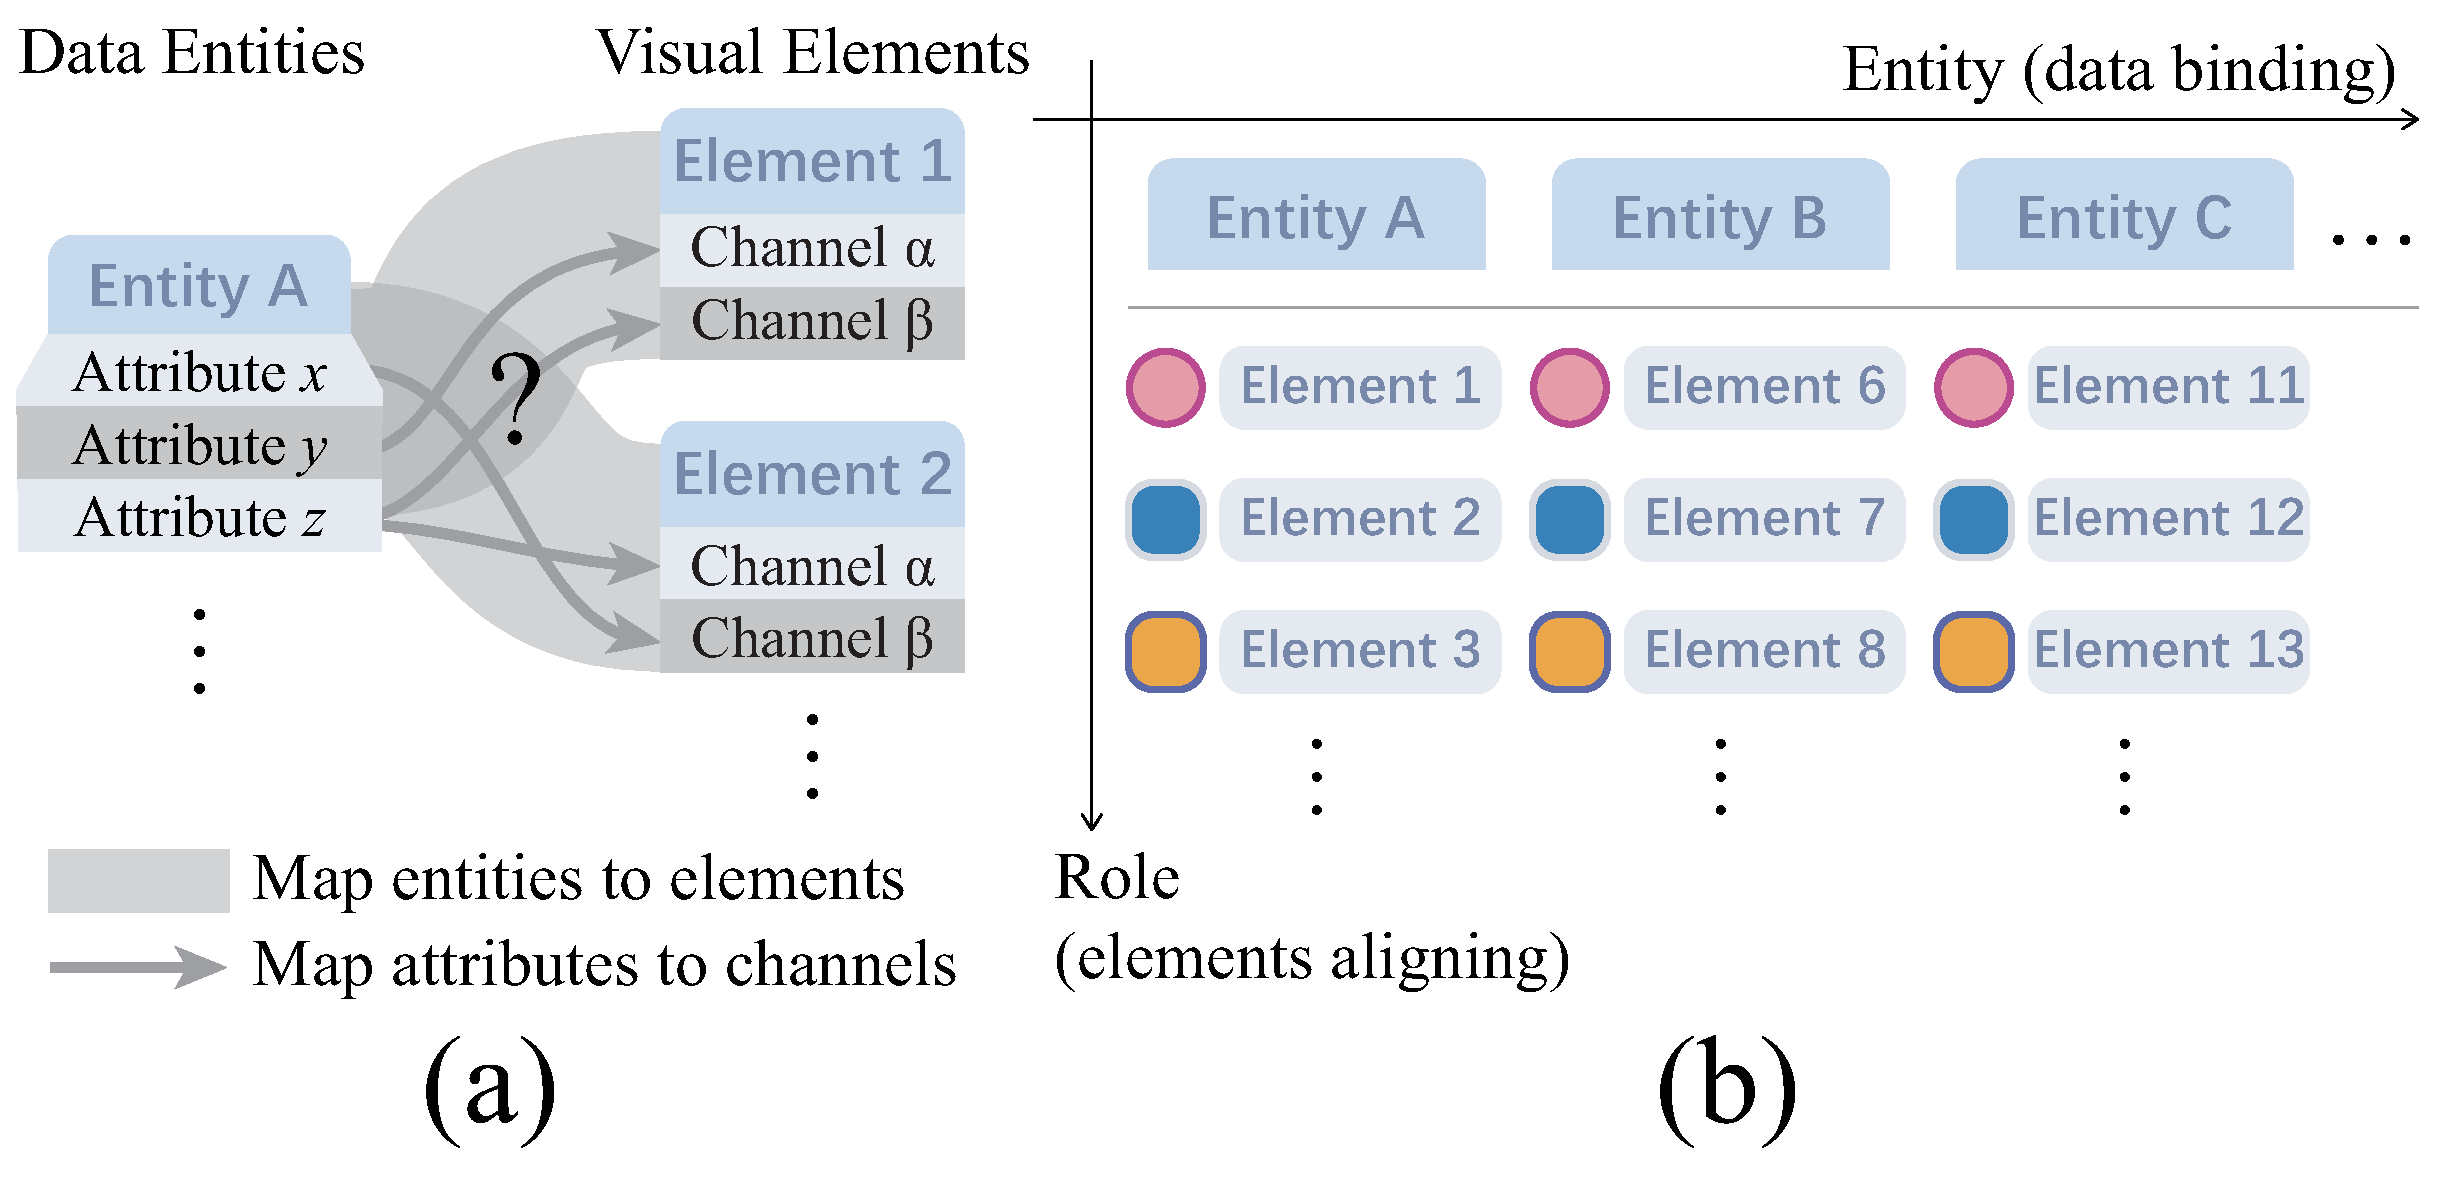
\includegraphics[width=1\columnwidth]{figures/ElementAligning.eps}
    \caption{(a) the target of our visual encoding detection technique; and (b) the effect of the data binding step and the elements aligning step.}
    \label{fig:ElementAligning}
\end{figure}

% xxxx 等人的工作为我们提供了一个良好的思路,但他们的工作存在一些限制
A tool proposed by Harper and Agrawala~\cite{DBLP:conf/uist/HarperA14} provides a creative perspective for visual encoding extraction.
Although their tool can be extended to support simple node-link diagrams (where each data entity is encoded into only one element), it still has several limitations:
\begin{compactenum}
% 1. 其需要创作者使用d3的数据绑定,才能发挥__data__的作用;使用其他工具,或者未将数据绑定到元素上时则无法使用该方法;
\item The data binding feature of D3 is required within the tool such that the ``\texttt{\_\_data\_\_}'' attribute of visual elements can be acquired by it. 
It cannot deal with SVG-format visualizations without data bound to visual elements.

% 2. 其只能检验属性和视觉通道之间是否存在线性映射或者类别性映射。
\item Only the linear mapping and the categorical mapping are supported, it cannot maintain situations where visual mappings are complex.
\end{compactenum}

% 我们针对节点链接图的场景,提出了一个数据绑定的策略,通过不断调整输入的数据,检查输出的变化,从而获取数据到svg元素之间的映射关系以及属性到视觉通道之间的映射方式,以解决以上两个问题。
For node-link diagrams, we introduce a new technique to solve such limitations.
The main idea of our technique is regarding the source code as a black box.
Our technique obtains mappings between data entities and visual elements by detecting changes of the output SVG after modifying the input graph data.
It overcomes the limitations by three steps (Figure~\ref{fig:VisualEncodings}):
(1) \textbf{Data binding} binds elements into different data entities.
(2) \textbf{Elements aligning} aligns elements according to their \textit{roles}. 
(3) \textbf{Encoding mapping} detects correlations between attributes, elements, and their visual channels.

\subsubsection{Data Binding} \label{sec:databinding}
To detect mappings between data entities and visual elements, 
we modify attribute values of data entities and record corresponding visual element changes.
Mappings between the entity and the changed elements are hence constructed.
However, directly modifying attributes may deform the attribute distribution, which can influence visual mappings, so that elements related to other data entities may also be changed.
For example, modifying attributes may broaden the attribute range and thus changes linear mappings defined by the attribute range.
We prevent it by only swapping attributes of two entities rather than modifying them, such that no new data is introduced and the distribution is preserved.
We take nodes for example.
Each node will be swapped with all the other nodes to make sure all elements belongs to it are detected.
Elements changed by each swapping correspond to two swapped nodes (Figure~\ref{fig:DataBinding} (b) and (c)).
For example, after swapping nodes B and C in Figure~\ref{fig:DataBinding} (b), elements 1 to 4 are changed.
All these changed elements correspond to nodes B and C, because only B and C are swapped.
After swapping the node B with the node D in Figure~\ref{fig:DataBinding} (c), elements 2 and 3 are changed twice (Figure~\ref{fig:DataBinding} (b) and (c)), thus they correspond to node B because only node B are changed twice.
To ensure all elements of node B are detected, we swap it with all the other nodes.
After swapping all nodes, the entire node-element mappings are constructed (Figure~\ref{fig:DataBinding} (d)), thus node entities are bound to their elements.
Mappings between Links with their elements are constructed in the same.
Because swapping two nodes may influence their related links, nodes' related elements can contain links' elements,
we remove links' elements from the node-element mappings.

\begin{figure}
    \centering
    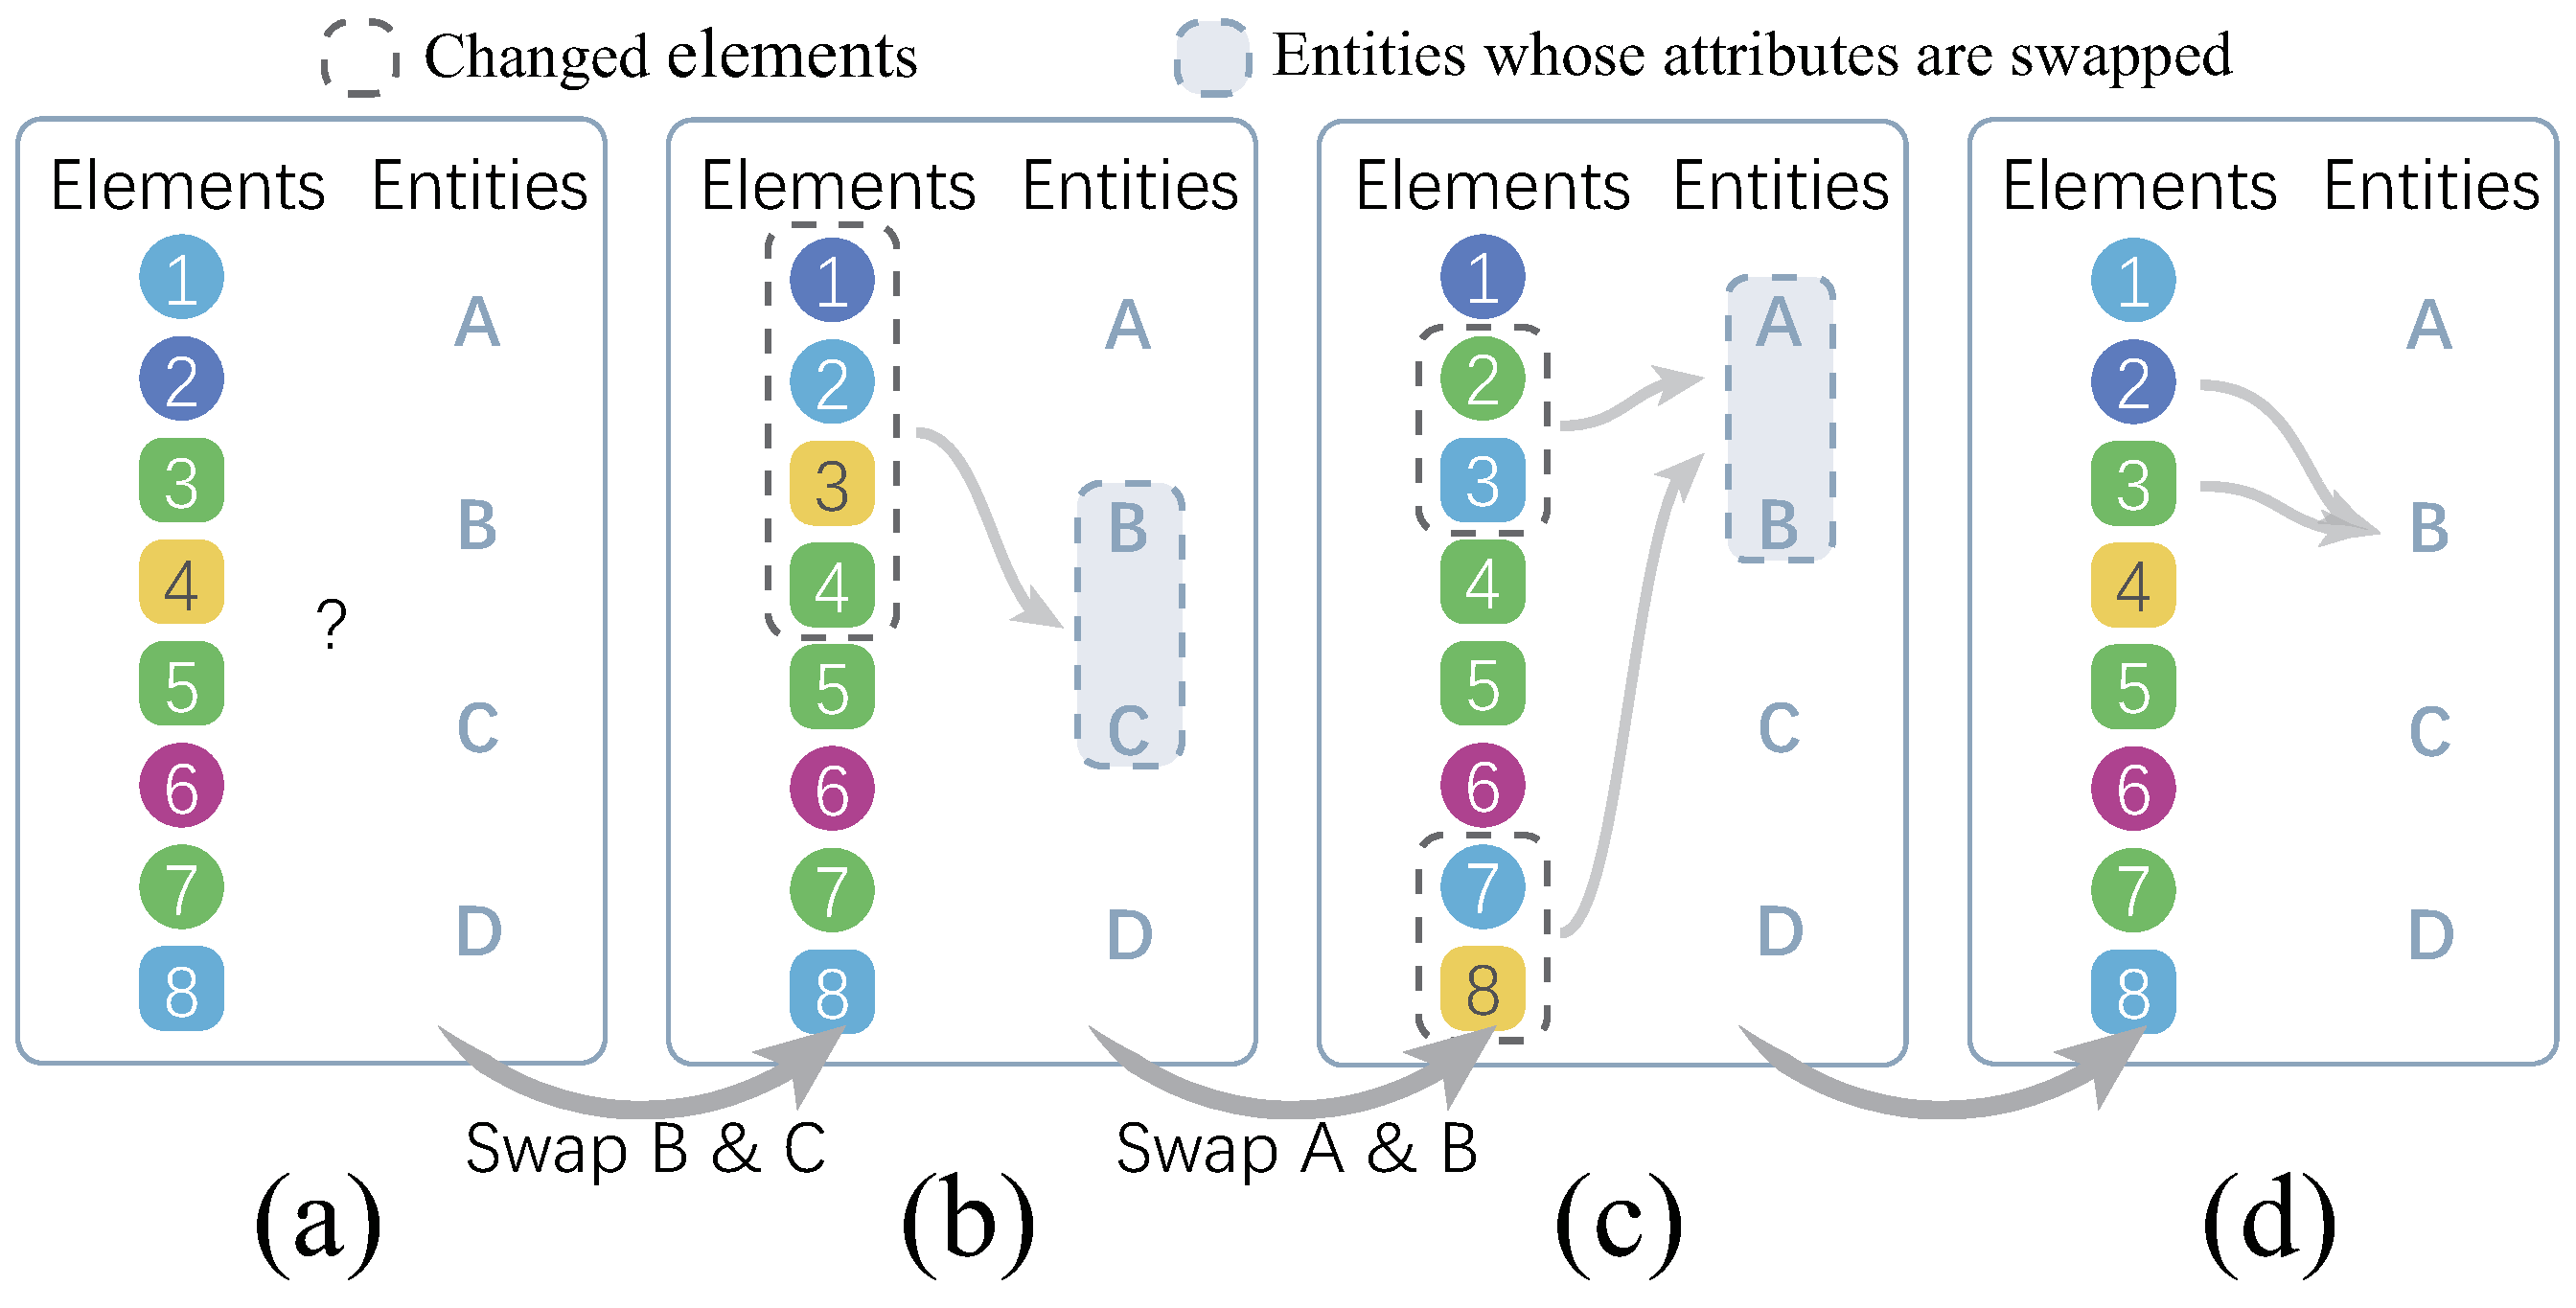
\includegraphics[width=1\columnwidth]{figures/DataBinding.eps}
    \caption{Data binding is achieved by swapping attributes of data entities. (a) Visual mappings between original visual elements and data entities are unknown. (b) After swapping attributes of entities B and C, the appearance of elements 1 to 4 is changed. Thus, entities B and C correspond to elements 1 to 4. (c) After swapping attributes of entities A and B, the appearance of elements 2, 3, 7, and 8 is changed. Thus, entities A and B correspond to these elements. (d) After swapping B with A and C, elements 2 and 3 are changed twice, we can map the entity B to elements 2 and 3.}
    \label{fig:DataBinding}
\end{figure}

\subsubsection{Elements Aligning}
% Different elements are aligned according to their roles (the vertical direction in Figure~\ref{fig:ElementAligning} (a)).
The data binding step only binds visual elements into different data entities (the horizontal direction in Figure~\ref{fig:ElementAligning} (b)).
The role of different elements within one data entity are undecided.
The role of a element can be defined as its affects of visualizing data attributes.
For the example in Figure~\ref{fig:VisualEncodings}, although both of the two inner rectangles are affected by the attribute \textit{y}, their affects are differently for the entire node (the left one encodes the first item in attribute \textit{y} and the right one encodes the second).
Whereas, affects of left rectangles across different nodes are same (they all encode the first item of $y$).
They should be aligned to clarify their roles (the vertical direction in Figure~\ref{fig:ElementAligning} (b)).
% The \textit{role} can be regarded as a function that takes data attributes as input and assign values for visual element channels.
Elements across different data entities are regarded as the same role if their encoding schemes are the same.
% Elements within the same role should appear exactly the same when their own nodes have exactly same attributes.
We test the consistency of encoding scheme between two elements by checking whether two elements appear consistently with same attributes.
Because we totally swap all the attributes of two entities, one entity before swapping is same to the other one after swapping.
We can examine the consistency of elements along with the swapping step.
For example, in Figure~\ref{fig:DataBinding} (b), after swapping entities B and C,element 1 appear same to element 2 before swapping (Figure~\ref{fig:DataBinding} (a)). Thus, element 1 and 2 can be aligned into the same role.
It clarifies the binding between data entities and visual elements, which is conductive to the subsequent steps.
% 这样做的意义:能够使得数据和可视化之间的绑定更加清晰,有利于后续步骤的进行。


\subsubsection{Encoding mapping}\label{sec:encodingmapping}
The previous two steps classify elements according to two dimension: entity and role.
We are able to answer \textbf{Q\ref{qstn:composition}}.
% 到此为止,我们已经已经知道每个实体是由哪些不同角色的元素组成,足够回答第一个问题
However, correlations between visual channels and data attributes are not determined.
% 我们继续以节点为例。
We continue to take nodes for example.
% 为了检验一个属性究竟被编码在了哪些视觉通道上,我们通过shuffle所有节点的某个属性,观察视觉通道发生的变化。
We map one attribute to its related visual channels by first shuffling values of the attribute of all nodes and then observing the changes of visual channels of elements.
% 变化可以被定义为,某个属性引起某些元素的某些视觉通道的变化。
One change can be defined as the difference of a certain \textit{visual channel} belongs a certain \textit{element} caused an \textit{attribute}, which can be formalized as:
\begin{equation}
    change := \{ attribute, element, channel \}
\end{equation}
% 然后我们根据不同的element角色,对这些发生的变化进行合并。
We merge those changes according to the role of element.
It generates more comprehensive mappings between attributes and visual channels for elements of different roles.
\textbf{Q\ref{qstn:encodings}} is solved.


To solve \textbf{Q\ref{qstn:correlation}}, we test correlations between attributes and visual channels.
Numerical and categorical attributes are supported.
And all the visual channels are regarded as numerical.
However, numerical data can be used as categorical data if there are only a few classes of values.
For example, natural numbers are usually used as categorical attributes such as labels, groups, and classes.
Thus, for the numerical data, we should compare the number of unique values and the number of their entries to determine whether it is numerical or categorical.
We set up a parameter $\alpha$, where the number of unique attribute values is less than $\alpha \%$ of the number of data entities, it is regarded as categorical.
We generate different correlations for different cases:
\begin{compactitem}
    \item The channel is categorical. The correlation is recorded and described by the channel's categories. For each category of the channel, we record value range of the attribute. % 我们记录了当视觉通道表达为这一类值的时候,属性的取值范围。
    If the value ranges of the attribute are intersected across different channel categories, we discard the correlation because it is ambiguous.
    \item Both the channel and the attribute numerical. We compute the Pearson's Correlation Coefficient and test whether the correlation is positive, negative, or uncorrelated with the generated p-value of the significance test. We take the attribute as the impact factor of the layout when the absolute value of the coefficient are larger than $\theta$ and the $p$-value of the significance test is less than $\alpha$. We set $\theta = 0.6$ and $\alpha = 0.05$ in default, they can be adjusted on demand.
    Both two parameters can be adjusted freely.
\end{compactitem}


\subsubsection {Template-based Textualization}
Nodes are described at first, followed by descriptions of links. 
% 为了标记模板中用于填充信息的部分,我们对这些位置进行了高亮。
To highlight the placeholders of templates that are used to fill in the information, we assign the \$ sign at the beginning of words that fill into these placeholders.

% 首先,我们需要描述数据实体被可视化为哪些视觉元素
We answer \textbf{Q\ref{qstn:composition}} with the elements that compose a node.
Because the shape (\texttt{tagName}) of elements may encode some attributes, we first describe the number of elements:
\textit{``Each \texttt{\$node} consists of \texttt{\$4} different elements''}. 
Then, elements of different roles are categorized and discussed. 
For each element, there are several visual channels encoding attributes.
We describe its shape first: \textit{``The \texttt{\$first} element is a \texttt{\$<rect>}''}.
If the shape is used to encode some attribute, the template turns to: \textit{``For the \texttt{\$second} element, its \texttt{\$tagName} is varying among multiple shapes: \texttt{\$<rect>}, \texttt{\$<ellipse>}, and \texttt{\$<circle>}''}.

For the case where the shape encodes nothing, we describe visual channel correlations one by one.
We first declare which attribute is encoded by which channel: \textit{``Its \texttt{\$fill} encodes the attribute \texttt{\$group}''} (to solve \textbf{Q\ref{qstn:encodings}}).
We describe their correlation to solve \textbf{Q\ref{qstn:correlation}}.
If the correlation is categorical-to-categorical, we describe different categories separately: \textit{``When the value of the attribute \texttt{\$group} is \texttt{\$2}, its \texttt{\$fill} turns to \texttt{\$darkorange (\#ff7f0e)}.''} (To describe a color, we find the most similar color from a pre-defined set of colors with 146 different names).
If the correlation is numerical-to-numerical, we describe whether the channel will increase or decrease with the increase of the attribute value: \textit{``The greater the attribute @value is, the \texttt{\$greater} its \texttt{\$stroke-width} is.''}.

And if the shape (\texttt{\$tagName}) of a element encodes some attributes, we first describe common channels shared by different shapes (e.g., fill, stroke, stroke-width, et cetera): \textit{``The \texttt{\$fill} of all these shapes encodes the attribute \texttt{\$group}''}.
Different shapes have different visual channels, we describe them separately: \textit{``When it turns to \texttt{\$<circle>}, its \texttt{\$r} encodes the attribute \texttt{\$degree}''}.

Examples of generated descriptions are referred in Figure~\ref{fig:BasicCases},~\ref{fig:NodeLineChartsCase},~\ref{fig:LinkBarsCase}.

\subsection{Interpreting Layout Intention}
Layouts of attributed graphs have been categorized into attribute-based layouts~\cite{} and topology-based layouts~\cite{} by Nobre et al.~\cite{DBLP:journals/cgf/NobreMSL19}.
Our technique focus on describing whether the layout is an attribute-based layout or a topology-based layout.
The core is to determine the type of the layout.
It contains two steps: 

\textbf{1) Capturing the position of each node;} To capture the position of each node, we compute a bounding box for elements detected in Section~\ref{sec:databinding}.
The bounding box of a node is the smallest rectangle that contains all elements of it.
We take the centroid of the bounding box as the position of the node.

\textbf{2) Determining the type of the layout.} 
The attribute-base category of layouts are defined as algorithms that mapping node attributes to the two dimensions (x and y) of the Cartesian coordinate. 
For each attribute of the node, we test whether it relates to the layout.
The test is similar to the correlation test in Section~\ref{sec:encodingmapping}.
Descriptions are also template-based: \textit{``The \texttt{\$x}-coordinate encodes the attributes \texttt{\$votes}''}.
If the test does not suggest any attribute as the impact factor, we begin to test whether it is topology-based.
For topology-based layouts, we assume that the euclidean distance between two nodes is influenced by their graph geodesic distance.
The Pearson correlation coefficient can also be used to test the correlation.
We assume that with the conditions that the Pearson correlation coefficient is larger than $\theta$ and $p$-value is smaller to $\alpha$, we can infer the layout is a topology-based layout.

Thus we first perform a pre-study to validate our hypothesis.
% 找N个不同的数据集(跨不同领域),找几种不同种类的拓扑based的layout;检验他们的pearson值,p值等等;比较它们在随机布局下的结果;
We prepare 15 different graph datasets from~\cite{DBLP:journals/tvcg/ZhuCHHLZ21}.
The number of their nodes varies from 72 to 1083 and the number of their links varies from 75 to 8677.
They are collected from diverse areas such as literature, music, research, social media, et cetera.
We layout them using 5 different kinds of topology-based layouts with default parameters: FM$^3$~\cite{hachul2004drawing}, Fruchterman-Reingold spring layout (F.R.)~\cite{DBLP:journals/spe/FruchtermanR91}, Stress Majorization (S.M.)~\cite{DBLP:conf/gd/GansnerKN04
}, Pivot MDS (PMDS)~\cite{DBLP:conf/gd/BrandesP06}, and Radial Tree layout (R.T.)~\cite{DBLP:conf/infovis/Jankun-KellyM03}.
% 我们还检验了随机布局是否也符合我们的假设
We also test whether the random layout conforms to our assumption.
We highlight cells where Pearson correlation coefficient is smaller than $\theta$ in Table~\ref{tab:pearson-correlation}.
$p$-values are all zero for the five layouts in all 15 datasets.
They suggest there is no correlation between the euclidean distance and the graph geodesic distance.
However, nine of 15 datasets with the random layout also produce $p$-values less than $\alpha$, which suggests they are significant.

% 这些基于拓扑的布局产生的节点位置,能够使节点间的欧式距离反应它们的拓扑距离。
Two tables suggest in most cases, the Euclidean distance between two nodes reflects their graph geodesic distance with topology-based layouts.
% 在大部分情况下,使用pearson 相关系数>0.6且p-value<0.05来检验是否该布局为拓扑布局是可行的。
Thus, it is feasible to check whether the layout is a topological layout with the first condition established (the Pearson correlation coefficient$>0.6$).

If the layout is topology-based, we only describe: \textit{``The layout is a topology-based layout, which means the greater the graph geodesic distance between two nodes is, the greater the euclidean distance between them is''}.
When the layout does not conform to the two categories, we describe that: \textit{``The layout is neither an attribute-based layout nor a topology-based layout.''}.

\begin{table}[ht]
\caption{\label{tab:pearson-correlation}Pearson correlation coefficients that test whether the euclidean distance between two nodes is related to their graph geodesic distance. 15 graphs and 6 different layouts are employed. Cells with coefficients less than $\theta$ are highlighted.}

\setlength{\tabcolsep}{1.5mm}{

% \resizebox{\textwidth}{15mm}{
\begin{tabular}{lllllll}
\hline
Dataset       & FM$^3$ & F.R.           & S.M.  & PMDS  & R.T.           & Random          \\ \hline
dwt\_72       & 0.894                 & 0.552          & 0.94  & 0.897 & 0.714          & \textbf{-0.003} \\
lesmis        & 0.804                 & 0.728          & 0.815 & 0.779 & \textbf{0.504} & \textbf{-0.03}  \\
bcsstk09      & 0.967                 & 0.610          & 0.971 & 0.947 & 0.754          & \textbf{-0.008} \\
cage8         & 0.658                 & 0.678          & 0.725 & 0.701 & \textbf{0.307} & \textbf{-0.002} \\
can\_96       & 0.835                 & 0.824          & 0.855 & 0.869 & \textbf{0.426} & \textbf{0.013}  \\
dwt\_1005     & 0.969                 & 0.561          & 0.974 & 0.972 & 0.623          & \textbf{0.007}  \\
dwt\_419      & 0.979                 & \textbf{0.391} & 0.987 & 0.987 & 0.775          & \textbf{-0.004} \\
grid17        & 0.968                 & 0.551          & 0.976 & 0.964 & 0.738          & \textbf{-0.007} \\
jazz          & 0.826                 & 0.821          & 0.813 & 0.786 & \textbf{0.297} & \textbf{0.004}  \\
mesh3e1       & 0.99                  & 0.502          & 0.996 & 0.995 & \textbf{0.465} & \textbf{0.002}  \\
netscience    & 0.901                 & 0.573          & 0.93  & 0.919 & 0.752          & \textbf{-0.018} \\
price\_1000   & 0.783                 & \textbf{0.376} & 0.808 & 0.786 & 0.727          & \textbf{-0.007} \\
rajat11       & 0.753                 & 0.670          & 0.868 & 0.847 & 0.618          & \textbf{-0.064} \\
soc-wiki-Vote & 0.798                 & 0.775          & 0.821 & 0.757 & \textbf{0.316} & \textbf{-0.01}  \\
visbrazil     & 0.937                 & 0.828          & 0.941 & 0.958 & 0.758          & \textbf{0.01}   \\ \hline
\end{tabular}}
\end{table}

% \begin{table}[ht]
% \caption{\label{tab:pearson-pvalue}Pearson p-value(TODO).}

% \setlength{\tabcolsep}{1.9mm}{

% \begin{tabular}{lllllll}
% \hline
% Dataset       & FM$^3$ & F.R. & S.M. & PMDS & R.T. & Random         \\ \hline
% dwt\_72       & 0                     & 0    & 0    & 0    & 0    & \textbf{0.842} \\
% lesmis        & 0                     & 0    & 0    & 0    & 0    & 0.021          \\
% bcsstk09      & 0                     & 0    & 0    & 0    & 0    & 0              \\
% cage8         & 0                     & 0    & 0    & 0    & 0    & 0.027          \\
% can\_96       & 0                     & 0    & 0    & 0    & 0    & \textbf{0.203} \\
% dwt\_1005     & 0                     & 0    & 0    & 0    & 0    & 0              \\
% dwt\_419      & 0                     & 0    & 0    & 0    & 0    & \textbf{0.111} \\
% grid17        & 0                     & 0    & 0    & 0    & 0    & \textbf{0.060} \\
% jazz          & 0                     & 0    & 0    & 0    & 0    & \textbf{0.421} \\
% mesh3e1       & 0                     & 0    & 0    & 0    & 0    & \textbf{0.604} \\
% netscience    & 0                     & 0    & 0    & 0    & 0    & 0              \\
% price\_1000   & 0                     & 0    & 0    & 0    & 0    & 0              \\
% rajat11       & 0                     & 0    & 0    & 0    & 0    & 0              \\
% soc-wiki-Vote & 0                     & 0    & 0    & 0    & 0    & 0              \\
% visbrazil     & 0                     & 0    & 0    & 0    & 0    & 0.025          \\ \hline
% \end{tabular}}

% \end{table}

\subsection{Interactive Descriptions}
Descriptions can be enhanced by interactions.
They are generated with corresponding elements.
For example, descriptions about nodes correspond to nodes related elements.
When audiences hover on one sentence of description, we highlight related elements to help user capture the target of the description.
We develop an interactive interface to support generating interactive descriptions (Figure~\ref{fig:interface}) with \ApproachName.
Creators can write visualization code in the Code Editor and input the graph data in the Data Editor.
\ApproachName~generates the visualization results and its corresponding interactive descriptions.


\begin{figure}[ht]
    \centering
    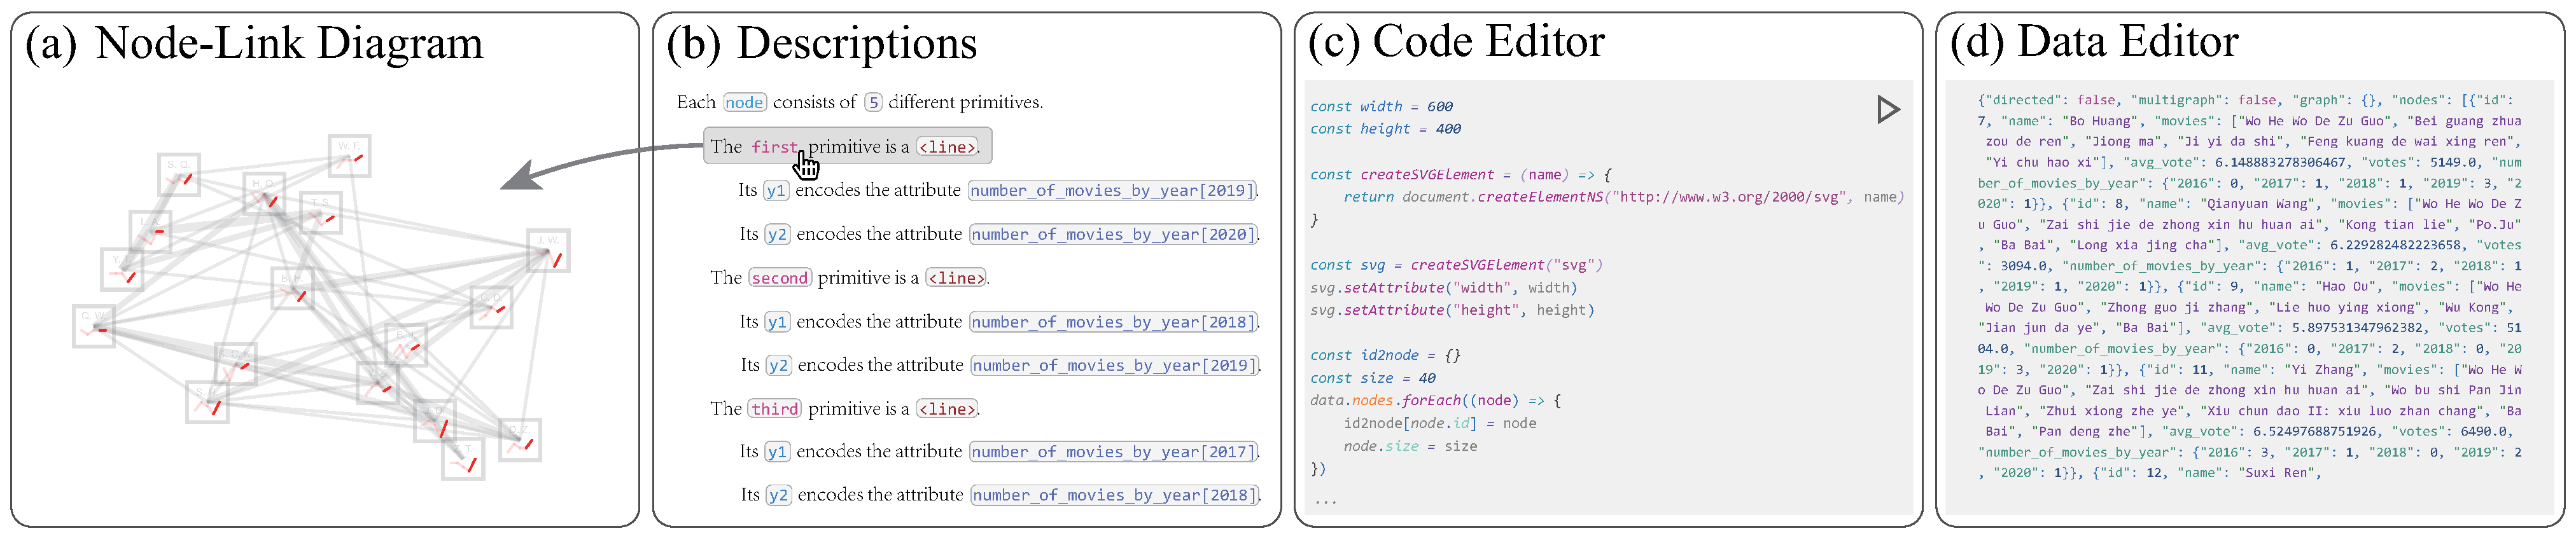
\includegraphics[width=1\columnwidth]{figures/interface.eps}
    \caption{The interface consists of four parts: (a) the node-link diagram view, (b) the descriptions view that shows the descriptions generated by \ApproachName, (c) the code editor view where creators can edit their visualization creation code, and (d) the data editor where creators input the graph data.}
    \label{fig:interface}
\end{figure}